\documentclass[11pt]{article}
\usepackage{natbib,mybigpackage}
\usepackage{algorithm}
%\usepackage{program}
%\usepackage{algpseudocode}
\usepackage{algorithmic}
\usepackage{listings}


\def\xbf{\mathbf{x}}
\def\zbf{\mathbf{z}}
\def\xibf{\mathbf{\xi}}
\title{Documentation: Assignment 7}
\author{Abhinav Gupta\
 150123001}
\begin{document}
\titlepage
\newpage

%\begin{enumerate}
[Q 1] Generate 50 randam numbers from geometric distribution of the form :
f(x; p) = pqi−1
i = 1, 2, · · · 0 < p < 1.
Draw the probability mass function
% \end{enumerate}

\noindent{Code: R}

\begin{lstlisting}
sample<-c()
pmf<-c()
pmf_data<-c()
p<-runif(1)
x<-c()
cat("Randomly generated probabilities \"p\" and \"q\" are: ",p," ",1-p," respectively !!\n")
q<-1-p
count<-50
for(i in 1:count){
	u<-runif(1)
	sample[i]<-floor(log(u)/log(q))+1
	pmf[i]<-q**(i-1)-q**i
	pmf_data[i]<-p*(q**(sample[i]-1))
	x[i]<-i
}
png("question1-pmf--perfect.png")
plot(x,pmf,col="red",main=paste("p = ", toString(p)))
png("question1-pmf-based_on_data.png")
plot(sample,pmf_data,col="green",main=paste("p = ", toString(p)))
cat("Mean is: ",mean(sample),"\n")
cat("Variance is: ",var(sample),"\n")

\end{lstlisting}

\noindent{\textbf{Output}:}
Randomly generated probabilities "p" and "q" are:  0.2086162   0.7913838  respectively !!\

Mean is:  4.1\

Variance is:  14.62245\


\noindent{\textbf{Observation}:}
%\begin{enumerate}
	Note that the cumulative probability\
	\begin{equation}
	P(X ≤ j−1) = 1−q^{(j−1)}\
	\end{equation}
	Random Number Generated \textbf{X=Int(log(U)/log(q)) + 1}.\

	\textbf{p: 0.2086162}\

	\textbf{Mean: 4.1}\

	\textbf{Variance: 14.62245}\

	\textbf{Graph: }\

%\end{enumerate}
  \begin{figure}[H]
  \centering
 \subfloat[pmf-Perfect Graph- Theoretical]{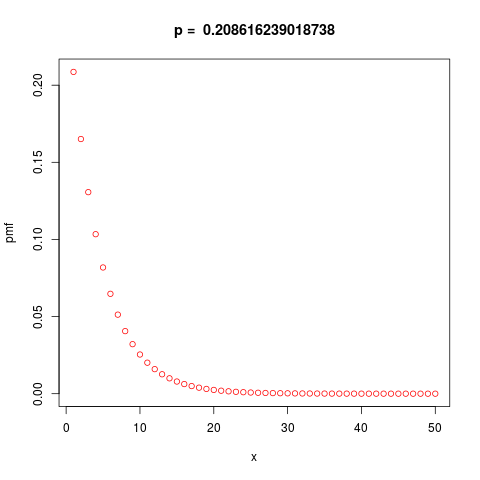
\includegraphics[width=1\textwidth]{question1-pmf-perfect.png}}\\
\end{figure}
  \begin{figure}[H]
  \centering
 \subfloat[pmf-Graph Based on Data - Observed]{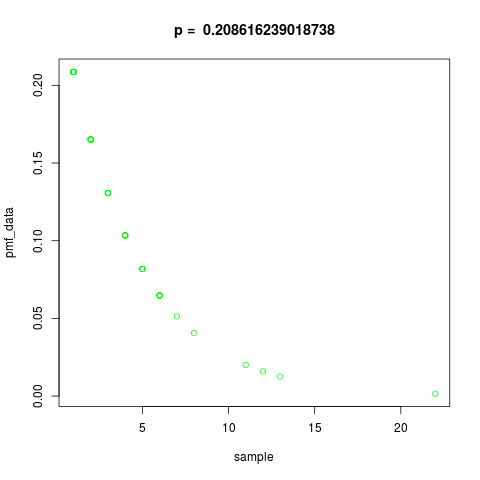
\includegraphics[width=1\textwidth]{question1-pmf-based_on_data.png}}\\
\end{figure}

%----------------------------------------------------------------------------------------------------------
%\begin{enumerate}
[Q 2] Generate 50 random numbers from poisson distribution with mean 2. Draw the probability
mass function and the cumulative distribution function.
%\end{enumerate}

\noindent{Code: R}
\begin{lstlisting}
sample<-c()
pmf<-c()
pmf_data<-c()
mean<-2
x<-c()
count<-50
for(i in 1:count){
	j<-0
	p<-exp(-1*mean)
	F<-p
	while(1){
		u<-runif(1)
		if(u<F){
			sample[i]<-j
			break
		}
		p<-(mean*p)/(j+1)
		F<-F+p
		j<-j+1
	}
	pmf[i]<-(exp(-1*mean)*(mean**(i-1)))/factorial(i-1)
	pmf_data[i]<-(exp(-1*mean)*(mean**(sample[i])))/factorial(sample[i])
	x[i]<-i
}
png("question2-pmf-perfect.png")
plot(x,pmf,col="red",main="pmf-perfect")
png("question2-pmf-based_on_data.png")
plot(sample,pmf_data,col="red",main="pmf-based_on_data")
png("question2-cdf.png")
plot(ecdf(sample),col="red")
cat("Mean is: ",mean(sample),"\n")
cat("Variance is: ",var(sample),"\n")
\end{lstlisting}

\noindent{\textbf{Output}:}
Theoretical Mean: 2\

Observed Mean is:  1.6\

Variance is:  0.9795918\

\noindent{\textbf{Observation}:}
%\begin{enumerate}
	\begin{equation}
	p_{i+1} =λ*p_i/(i+1) 
	\end{equation}
	\textbf{Observed Mean: 1.6}\

	\textbf{Variance: 0.9795918}\

	\textbf{Graph: }\


%\end{enumerate}
\begin{figure}[H]
  \centering
 \subfloat[pmf-Perfect Graph- Theoretical]{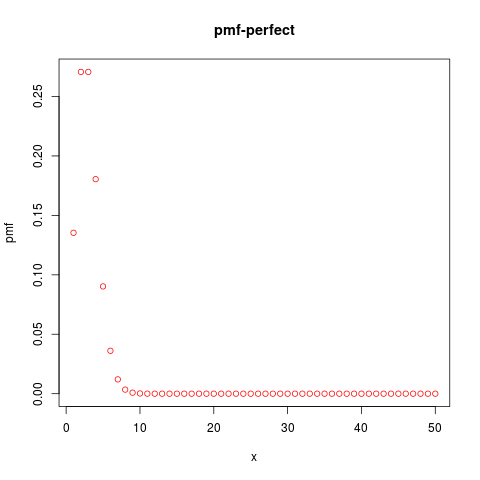
\includegraphics[width=1\textwidth]{question2-pmf-perfect.png}}\\
\end{figure}
\begin{figure}[H]
  \centering
 \subfloat[pmf-Graph Based on data- Observed]{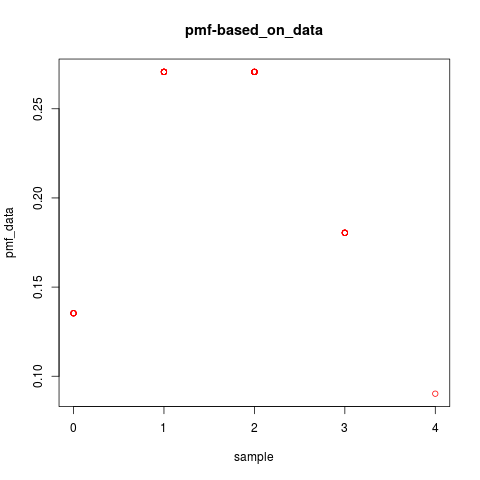
\includegraphics[width=1\textwidth]{question2-pmf-based_on_data.png}}\\
\end{figure}
\begin{figure}[H]
  \centering
 \subfloat[CFD]{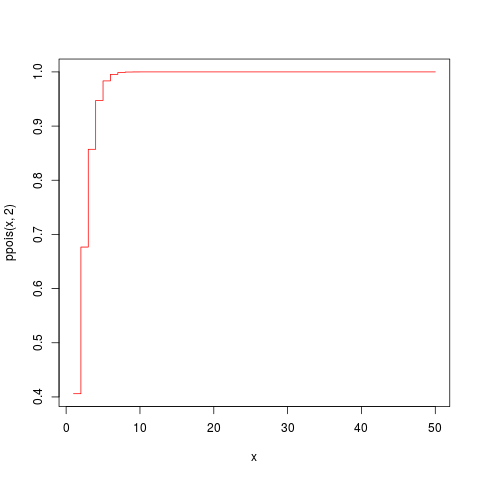
\includegraphics[width=1\textwidth]{question2-cdf.png}}\\
\end{figure}

%---------------------------------------------------------------------------
%\begin{enumerate}
[Q 3] Draw the histogram based 50 generated random numbers from the mixture of two
Weibull distributions :
f(x; β1, θ1, β2, θ2, p) = pf1(x; β1, θ1) + (1 − p)f2(x; β2, θ2)
where f1(·) and f2(·) are two Weibull distributions of the form : f(x; β, θ) = βθβx
β−1
e
−(θx)
β
where, β1 = 2, θ1 = 1, β2 = 1.5, θ2 = 1, p = 0.4
%\end{enumerate}

\noindent{Code R: }

\begin{lstlisting}
theta1<-1
theta2<-1
beta1<-2
beta2<-1.5
p<-0.4
q<-0.6
first<-function(u){
	return (((-1*log(u))**(1/beta1))/theta1)
}
second<-function(u){
	return (((-1*log(u))**(1/beta2))/theta2)
}
count<-50
sample<-c()
for(i in 1:count){
	u1<-runif(1)
	x1<-first(u1)
	x2<-second(u1)
	u2<-runif(1)
	if(u2<p)
		sample[i]<-x1
	else
		sample[i]<-x2
	cat(sample[i],"\n")
}
hist(sample)
cat("Mean is: ",mean(sample),"\n")
cat("Variance is: ",var(sample),"\n")

\end{lstlisting}


\noindent{\textbf{Output: }}

\textbf{Mean: 0.8324047}\

\textbf{Variance: 0.2156945 }\

\noindent{\textbf{Observation}:}
%\begin{enumerate}
	CDF of Weibull Distribution:\
	\begin{equation}
	F(x)= 1-e^{-(theta*x)^{beta}}
	\end{equation}

step 1: genrate a random number U1
step 2: generate X1 and X2 from weibull distributions given.
step 3: if U2 < p, set X = X1.
step 4: else if U > p , set X = X2.


	\textbf{Observed Mean: 0.8324047}\

	\textbf{Variance: 0.2156945}\

	\textbf{Graph: }\


%\end{enumerate}
\begin{figure}[H]
  \centering
 \subfloat[Histogram of mixed distribution]{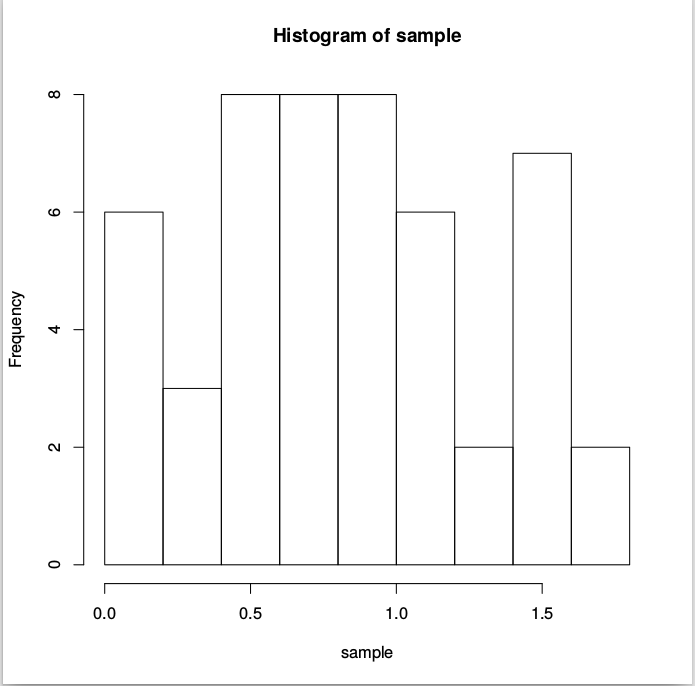
\includegraphics[width=1\textwidth]{question3-histogram.png}}\\
\end{figure}
\end{document}

